% Appendix Template

\chapter{Appendix 3} % Main appendix title

\label{appendix3} % Change X to a consecutive letter; for referencing this appendix elsewhere, use \ref{AppendixX}

\lhead{Lighthouse result graphs} % Change X to a consecutive letter; this is for the header on each page - perhaps a shortened title

\section{Lighthouse result graphs}

\begin{figure}[!h]
	\centering
	\begin{adjustbox}{width=\textwidth,totalheight=0.7\textheight}
		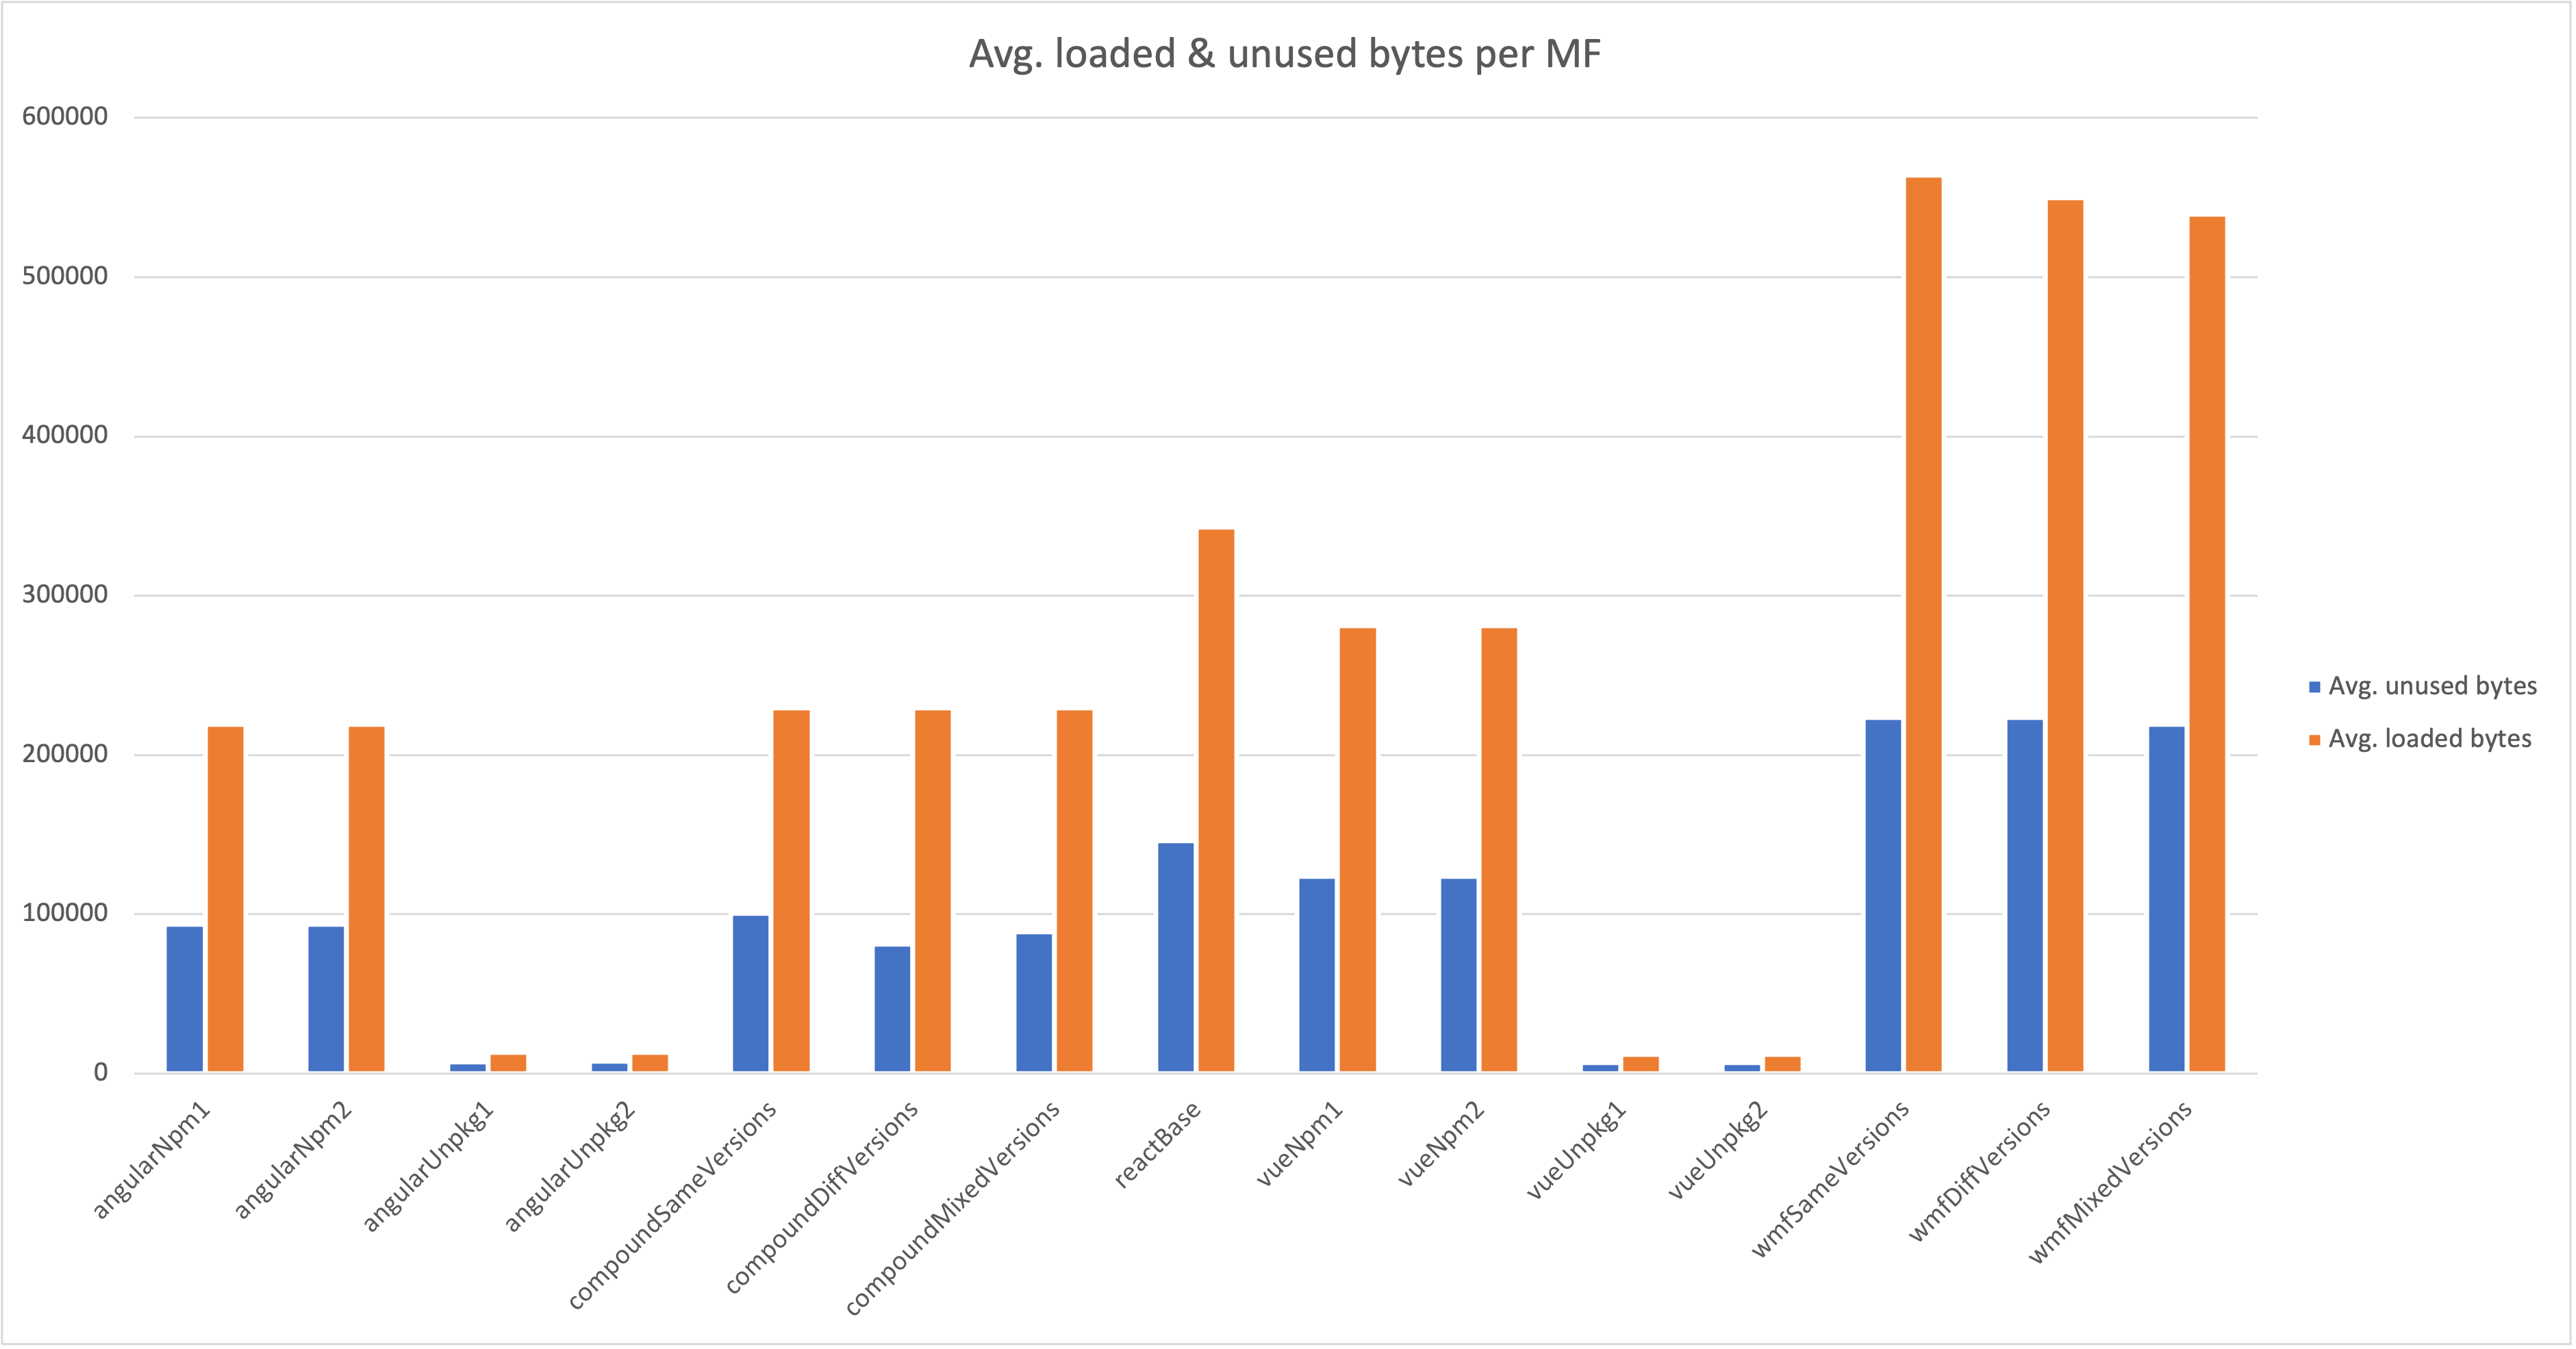
\includegraphics[angle=90]{Figures/avg_unsed_imported_mfe_1.png}
	\end{adjustbox}
	\caption{Bar chart for results taken from the Lighthouse reports, containing the imported and unused bytes per single MF}
	\label{fig:appendix_3_1}
\end{figure}
\newpage
\begin{figure}[!h]
	\centering
	\begin{adjustbox}{width=\textwidth,totalheight=\textheight}
		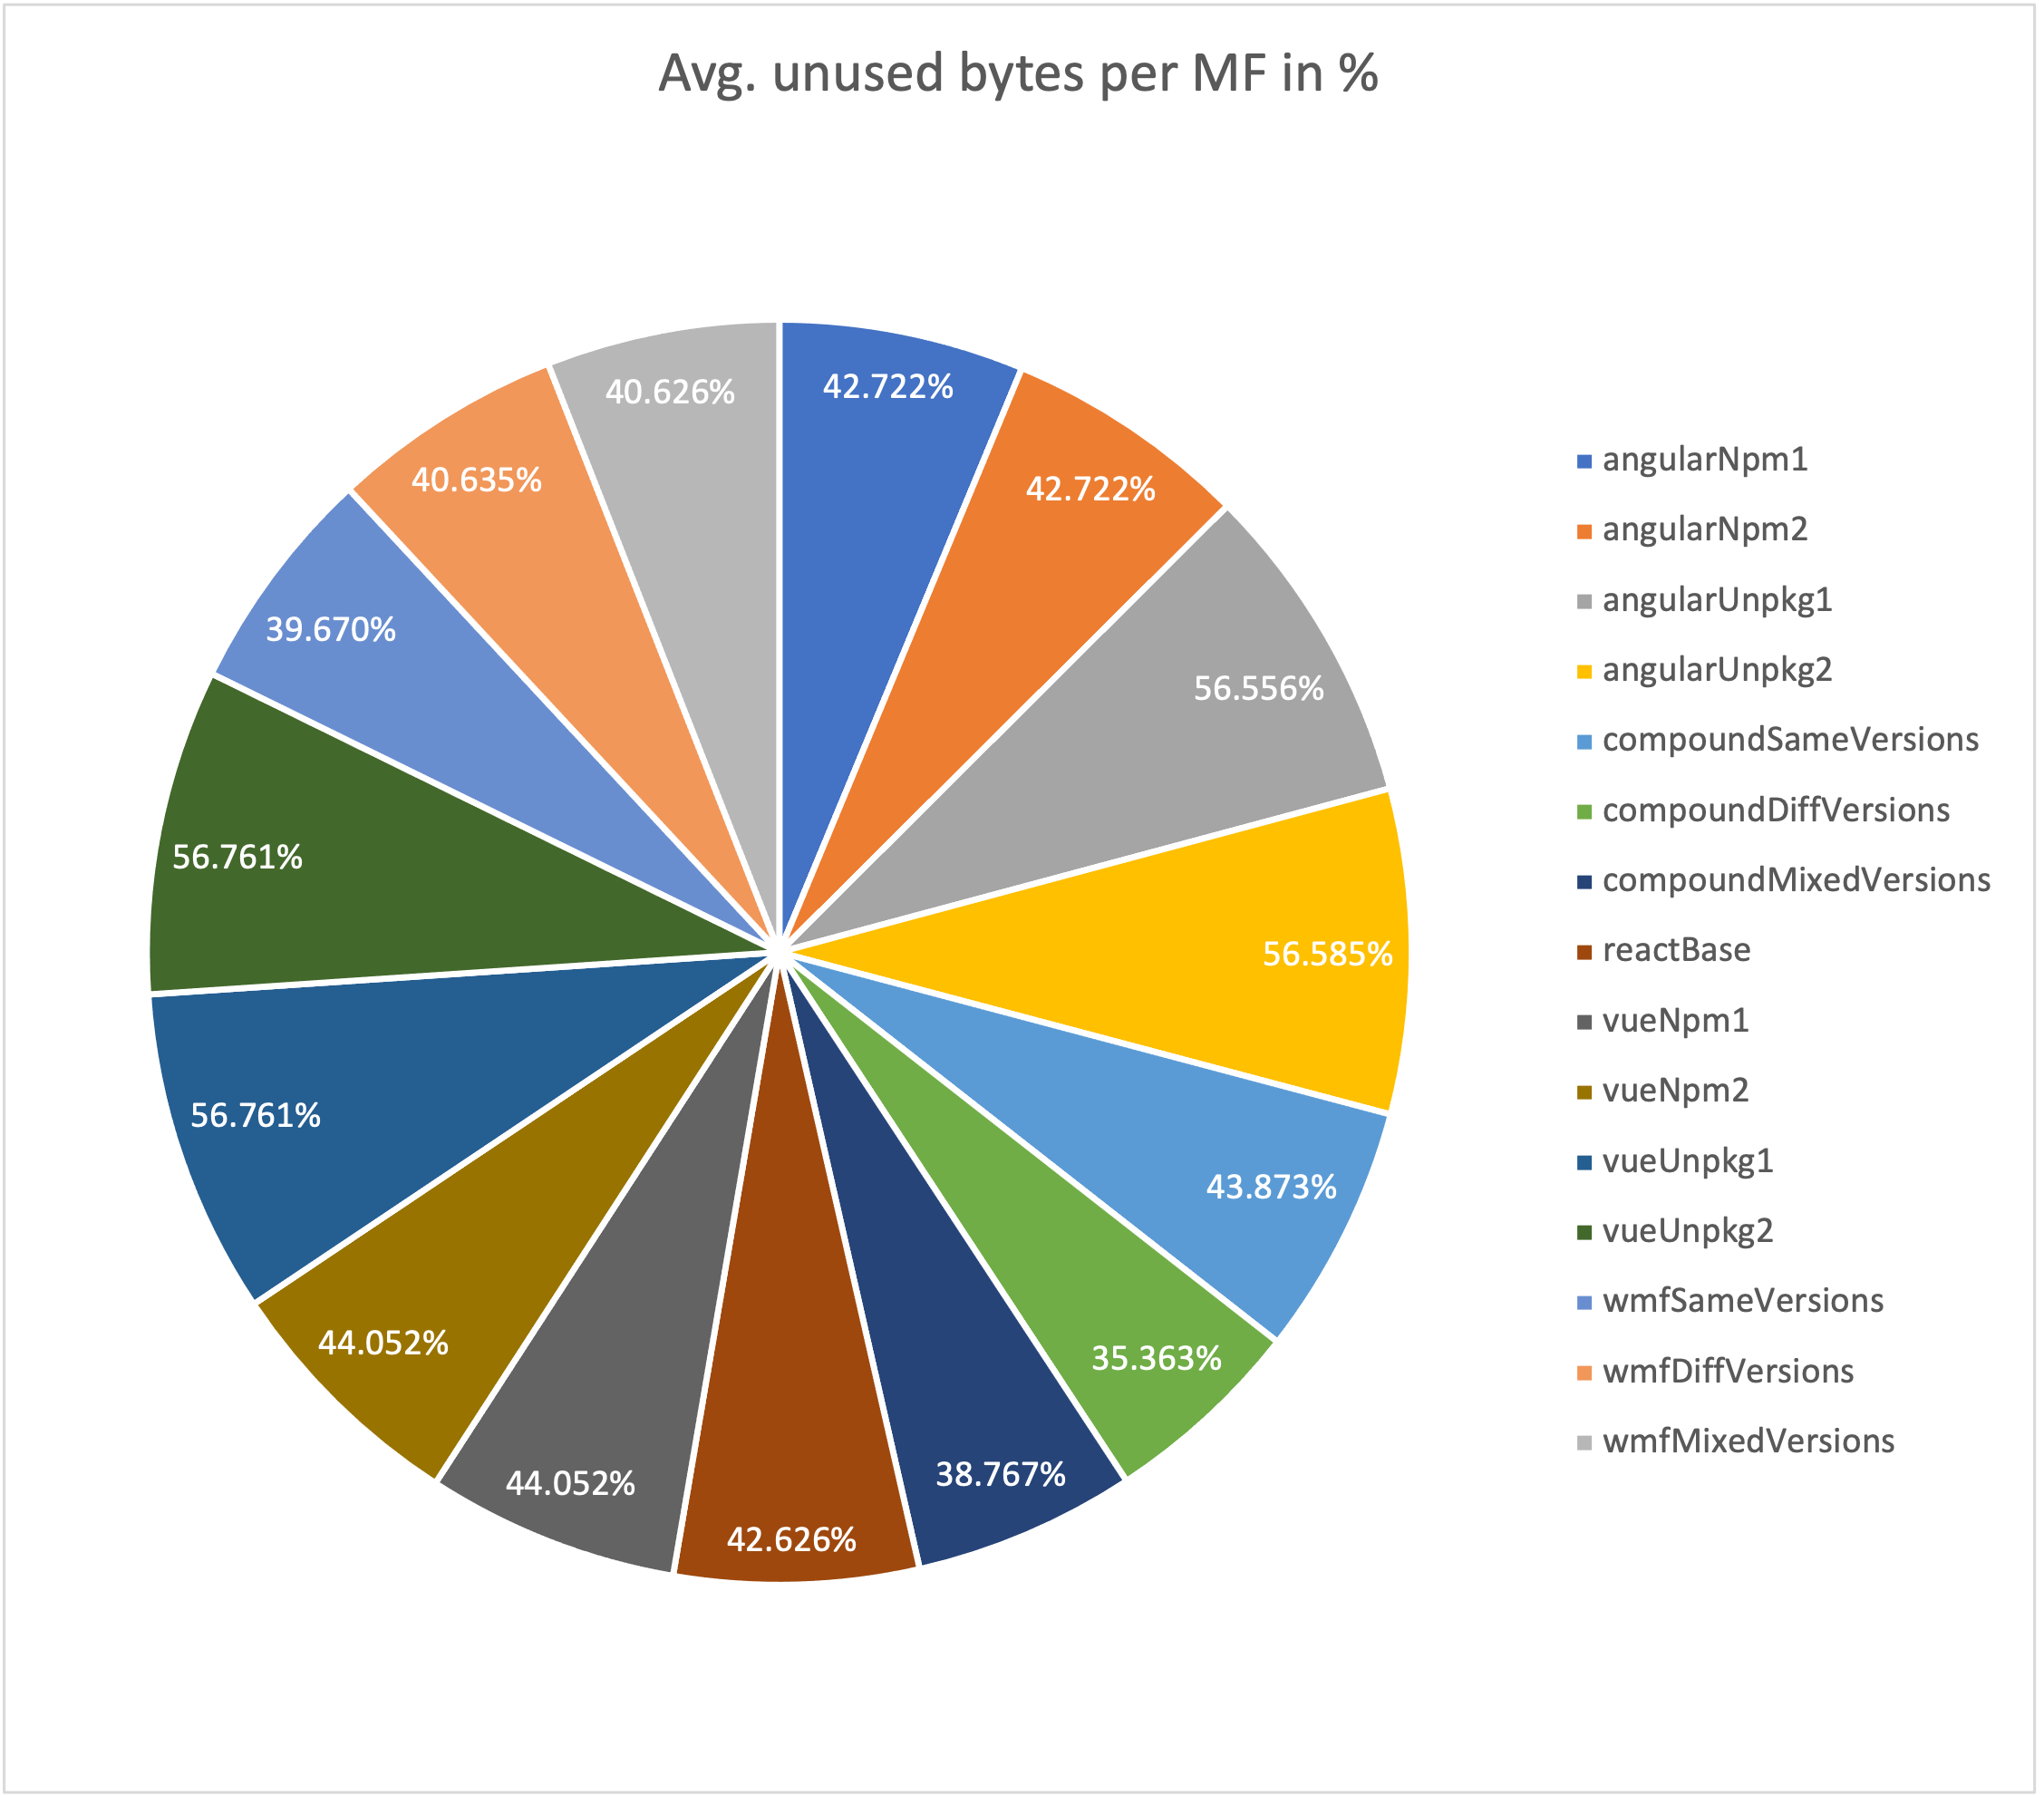
\includegraphics[angle=90]{Figures/avg_unsed_imported_mfe_2.png}
	\end{adjustbox}
	\caption{Pie chart for results taken from the Lighthouse reports, containing the unused bytes per single MF in \%}
	\label{fig:appendix_3_2}
\end{figure}
\newpage
\begin{figure}[!h]
	\centering
	\begin{adjustbox}{width=\textwidth,totalheight=\textheight}
		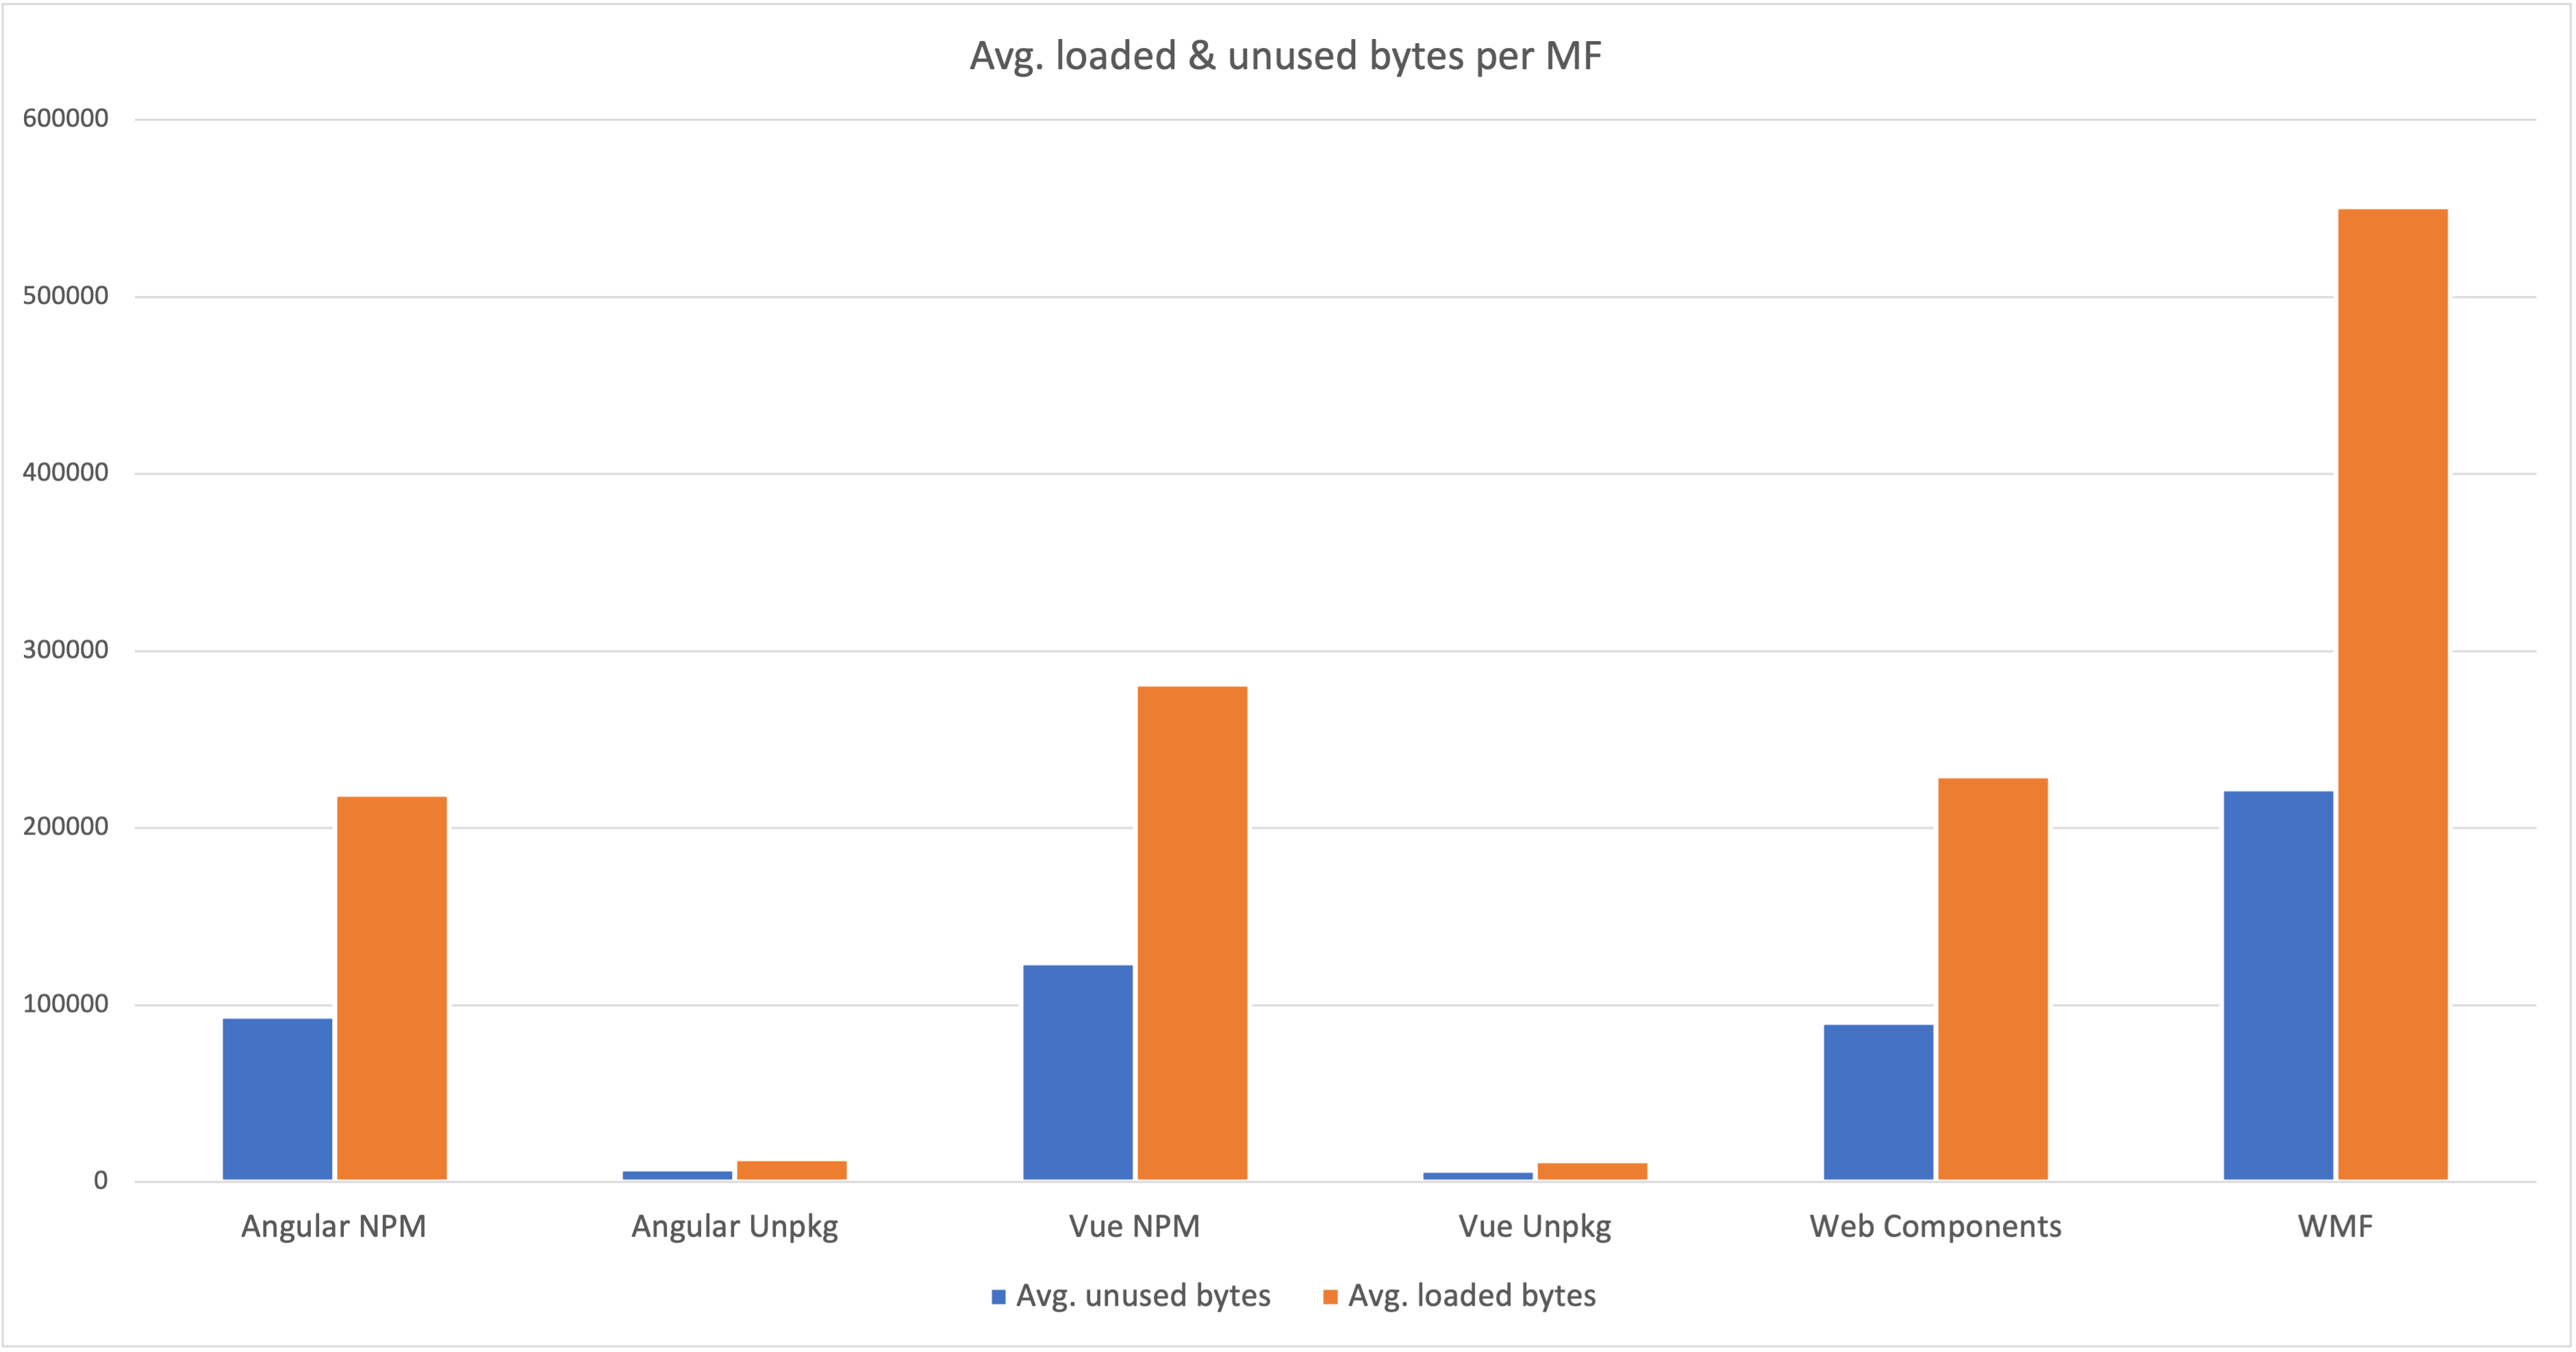
\includegraphics[angle=90]{Figures/avg_unsed_imported_1.png}
	\end{adjustbox}
	\caption{Bar chart for results taken from the Lighthouse reports, containing the imported and unused bytes per landscape}
	\label{fig:appendix_3_3}
\end{figure}
\newpage
\begin{figure}[!h]
	\centering
	\begin{adjustbox}{width=\textwidth,totalheight=\textheight}
		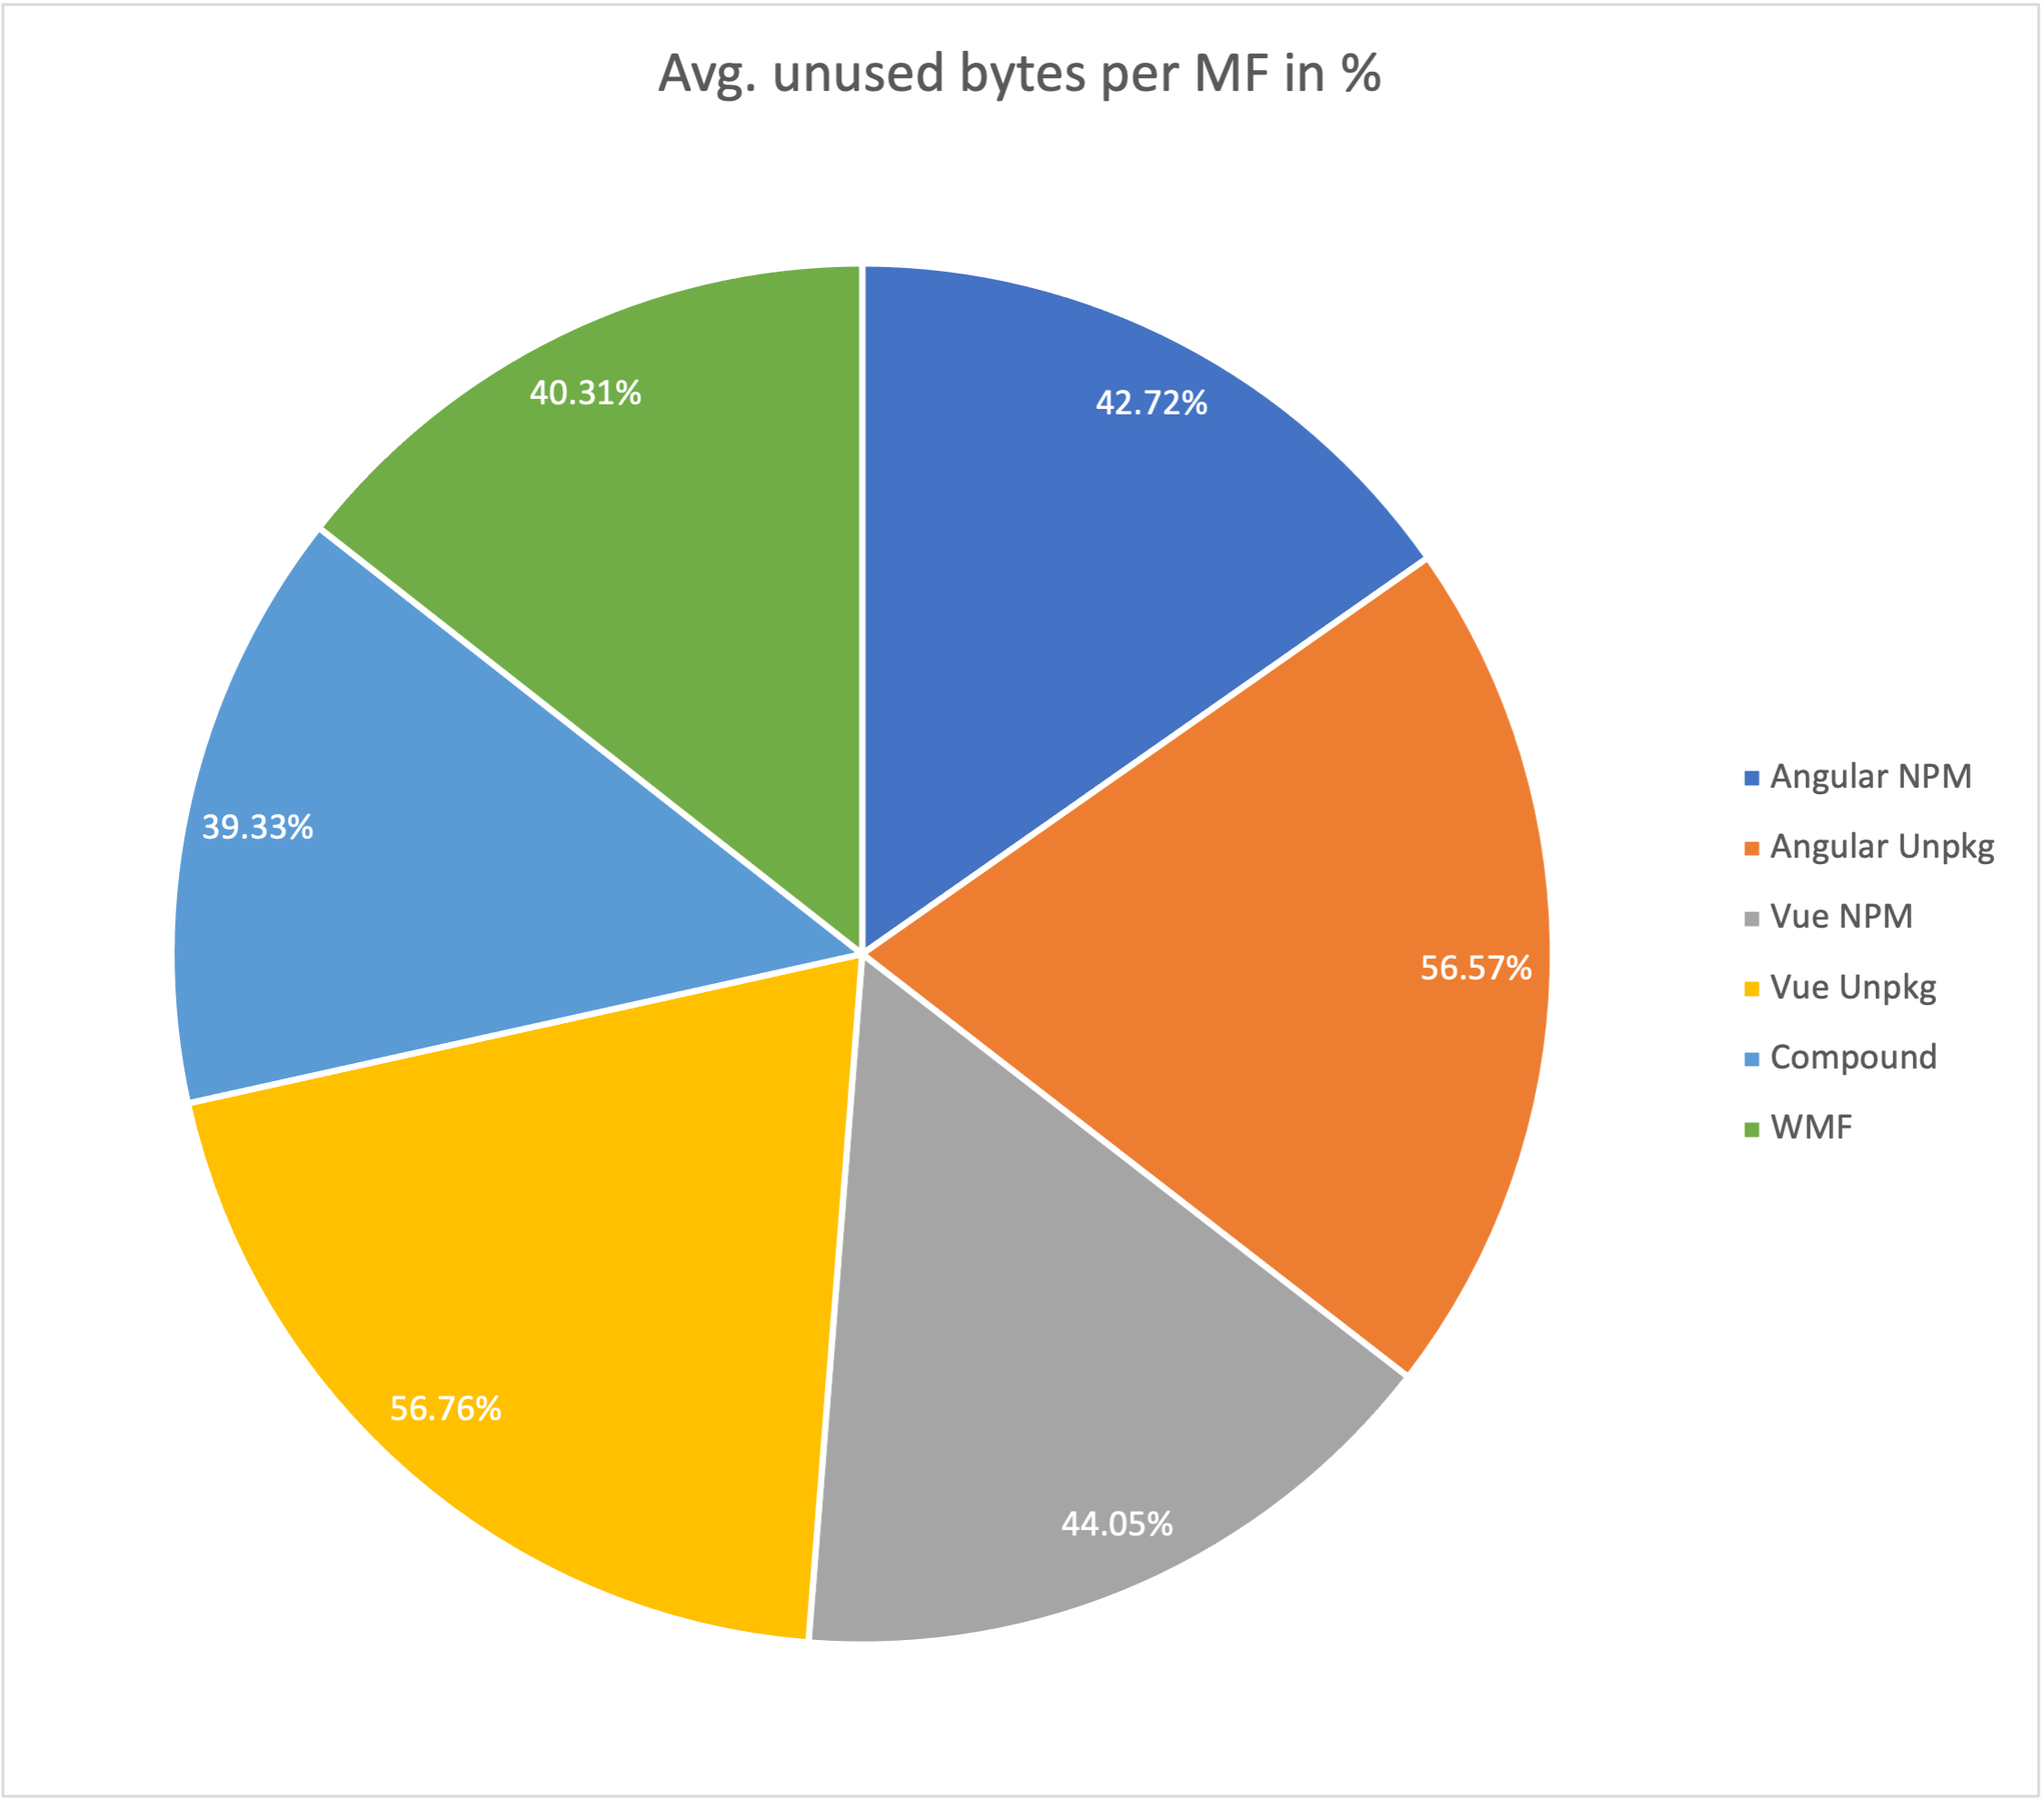
\includegraphics[angle=90]{Figures/avg_unsed_imported_2.png}
	\end{adjustbox}
	\caption{Pie chart for results taken from the Lighthouse reports, containing the unused bytes per landscape in \%}
	\label{fig:appendix_3_4}
\end{figure}